
\section{JPEG Image Compression (ms)}
\label{jpeg_image_compression}
\subsection{Introduction}
The images obtained from a camera will generally be in the JPEG image format
according to the 
EXIF (Exchangeable image file format for digital still cameras)
 (Exif Version 2.2).\cite{exif_std} 
JPEG is a form of image compression standard named after its developers, 
the Joint Photographic Experts Group. \cite{winzip_jpeg_compression}
This section will provide a quick overview of the JPEG image compression algorithm
and attempt to explain the information available by
analysing the JPEG file structure.

\subsection{JPEG Compression Process}

The JPEG compression algorithm uses 8 
stages to compress an image: \cite{hass_impulse_jpeg}

\subsubsection{Stage 1: Colour Space Conversion}
The image undergoes chroma subsampling from the 
RGB colour model to a 4:2:2 or a 4:2:0 YCbCr colour model. 
Both subsampling patterns are approved by the
EXIF (Exchangeable image file format for digital still cameras)
and the pattern used is dependant on the camera's specifications. 
(see section \ref{sec:colour_space_conversion})

\subsubsection{Stage 2: Block Segmentation}
The image is then separated into 8x8 or 16x16 pixel blocks,
called MCUs (Minimum Coded Unit) 
depending on whether the image has been chroma
subsampled to a 4:2:2 or 4:2:0 model respectively. \cite{exif_std}

\subsubsection{Stage 3: Discrete Cosine Transform}
The image is transformed from a spatial domain 
representation to a frequency domain representation
using the Discrete Cosine Transform. \cite{hass_impulse_jpeg}
(see section \ref{transfom_base})

\subsubsection{Stage 4: Quantization}
Using the wave equations from the DCT step,
the algorithm sorts them from low-frequency
components (gradual colour changes) to 
high-frequency components (sudden colour changes),
from the top left to the bottom right corner of the image.
The algorithm discards the high-frequency details
due to the human eye not recognizing them as
well as low-frequency details. This is done through 
division of all DCT wave equation 
coefficients using a quantization table and
then rounding the result to the nearest integer.
This quantization table differs between
the majority of digital cameras and 
software packages.\cite{hass_impulse_jpeg}

\subsubsection{Stage 5: Zigzag Scan}
The matrix obtained through quantization is
then re-ordered from the top-left corner into a 
64-element vector in a zig-zag pattern.
This is done to ensure that the high-frequency
components which are most likely to round to
zero after quantization, make up the lower
right hand part of the matrix.

\begin{figure}[!hbtp]
\begin{center}
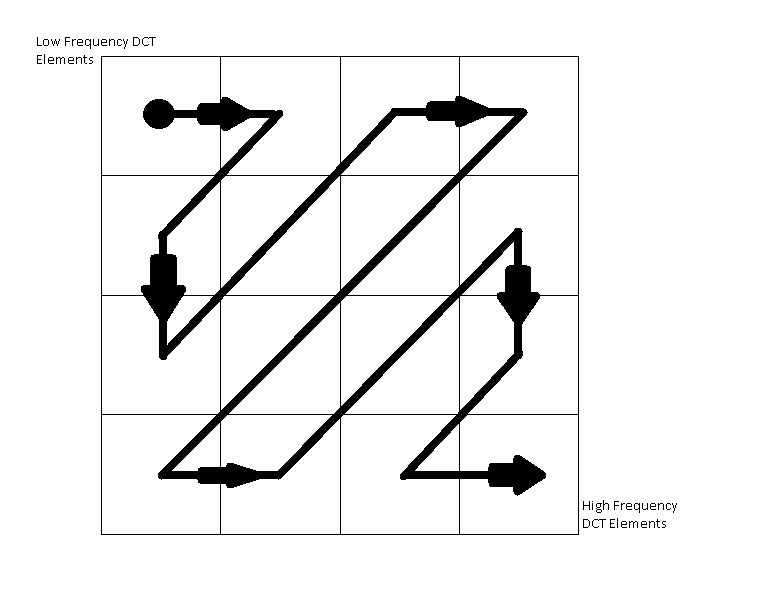
\includegraphics[scale=1]{figures/jpegzigzag.png} 
\end{center}
\caption{Example ofa zig zag scan \cite{hass_impulse_jpeg}}
\end{figure}

\subsubsection{Stage 6: DPCM on DC components}
DPCM is known as Differential Pulse
Code Modulation. It is the process of
calculating the block-to-block average difference
of the DC components across the entire MCU block
and encoding the average as a change from the 
previous block's value.\cite{hass_impulse_jpeg}

\subsubsection{Stage 7: RLE on AC components}
RLE is known as Run Length Encoding. It is the process of
storing each value of the AC components of the
64-element vector with the number of zeros
preceding it for the purposes of the final stage.\cite{hass_impulse_jpeg}

\subsubsection{Stage 8: Entropy Coding/ Huffman Coding}
Finally, a dictionary representing commonly used value strings with
shorter code is created. Common string and patterns
are represented by short codes while less frequently
used strings are represented with longer codes.
(see section \ref{sec:general_huff})

\subsection{JPEG Structure}
A JPEG file can be separated into two main parts. 
The first part of the JPEG file is composed of segments containing information concerning 
various properties of the image which must be read in order to display the image from its compressed form. 
The number of segments within one JPEG file varies from picture to picture.
The second part contains the entropy-encoded image data, which can be decoded using the information provided from the headers of the file.  

\subsubsection{JPEG Segments}
The JPEG headers are capable of storing most of the metadata related to an image, not all of which is necessary for the decompression of the image. 
The following headers are those which contain all the information necessary for 
a successful decompression of the JPEG image, as well as those which can be found in all JPEG images.
%% The SOI (Start Of Image) and APP (JFIF application) segments are recorded first, in that order.
%% These segments are followed by the DQT (Define Quantization Table(s)), DHT (Define Huffman Table(s)), and SOF (Start Of Frame) segments,
%%in any order depending on the image. 
%%The SOS (Start Of Scan) and entropy- encoded data are 
%%stored afterwards and the image ends with the EOI (End Of Image) segment.

The table below details some important segments which are necessary for the image
to be properly displayed: \cite{exif_std}

\begin{table}[!hbtp]
	\caption{JPEG File Layout}
	\centering
	\begin{tabular}{ | p{1.5cm} | p{3cm} | p{2cm} | p{2.8cm} | }
	\hline
	\textbf{Segment Name} & \textbf{Marker Name} & 
	\textbf{Marker Code} & \textbf{Description} \\ \hline
	SOI & Start Of Image & 0xD8 & Start of compressed image data\\ \hline
	APP\emph{n} & Application Segment \emph{n} & 0xE\emph{n} & Exif application information segment\\ \hline
	DQT & Define Quantization Table(s) & 0xDB & Quantization table definition.\\ \hline
	DHT & Define Huffman Table(s) & 0xC4 & Huffman table definition.\\ \hline
	SOF & Start Of Frame & 0xC0 & Frame parameter data\\ \hline
	SOS & Start Of Scan & 0xDA & Scan parameter data\\ \hline
	\end{tabular}
\end{table}

The entropy-encoded image data appears after the SOS segment,
right before the EOI header marker.

For information concerning the actual content of each of the 
JPEG segments, please refer to the appendix \ref{chap:jpeg-segment-contents}.

\subsubsection{Entropy-encoded image data}
\label{sec:entropycrho}

The image data is received chrominance pixel by chrominance pixel. 
The first bytes received are the luma values of the individual image pixels. 
In the case of JPEG images, they are received from left to right, top to bottom, moving horizontally before vertically. 
The luma values are then followed by the Cb and Cr values of the top-left pixel, in that order. 
After all the data for a single chrominance pixel has been sent (6 bytes) those of the next chrominance pixel are sent in the same format, 
read in the same order as the image pixels within one chrominance pixel. This continues until the EOI marker is found.
